\chapter{Ejemplos prácticos}

\section{Introducción}

Este capítulo presenta un ejemplo práctico completo que demuestra el uso de SimAS 3.0 para crear una gramática de contexto libre y realizar un análisis sintáctico descendente. El ejemplo seguirá todo el flujo de trabajo desde la creación de la gramática hasta la simulación del análisis, mostrando las capacidades completas de la aplicación.

El ejemplo utiliza una gramática para declaraciones de variables que permite comprender los conceptos fundamentales del análisis sintáctico descendente, incluyendo la construcción de conjuntos PRIMERO y SIGUIENTE, la generación de tablas predictivas, y la simulación paso a paso del análisis.

\section{Creación de una gramática de contexto libre}

En esta sección se detalla el proceso completo de creación de una gramática utilizando el editor de SimAS 3.0. El ejemplo utiliza una gramática para declaraciones de variables que permite definir variables de tipo entero y flotante.

\subsection{Acceso al editor}

Para comenzar, accedemos al editor de gramáticas desde el menú principal, como se muestra en la figura \ref{fig:ejemplo_menu}.

\needspace{8cm}
\begin{figure}[H]
    \centering
    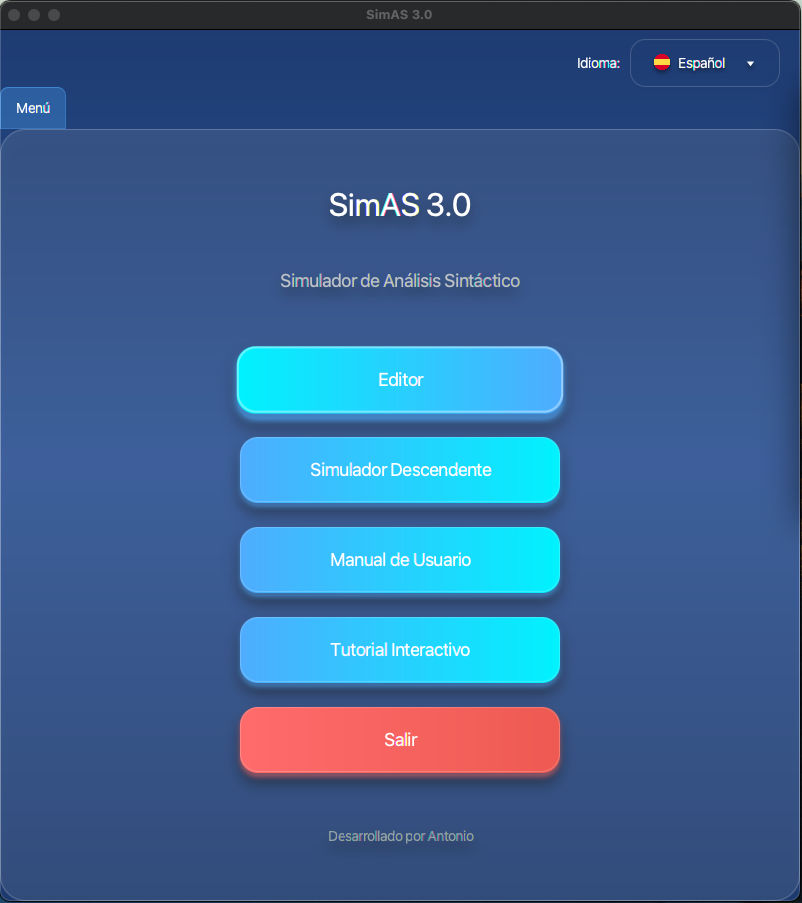
\includegraphics[width=0.9\textwidth]{figuras/ejemplo_practico/menu.png}
    \caption{Acceso al editor desde el menú principal}
    \label{fig:ejemplo_menu}
\end{figure}

\subsection{Paso 1: Datos de la gramática}

El primer paso consiste en definir los datos básicos de la gramática. En la figura \ref{fig:ejemplo_editor_paso1} se muestra la configuración inicial:

\needspace{8cm}
\begin{figure}[H]
    \centering
    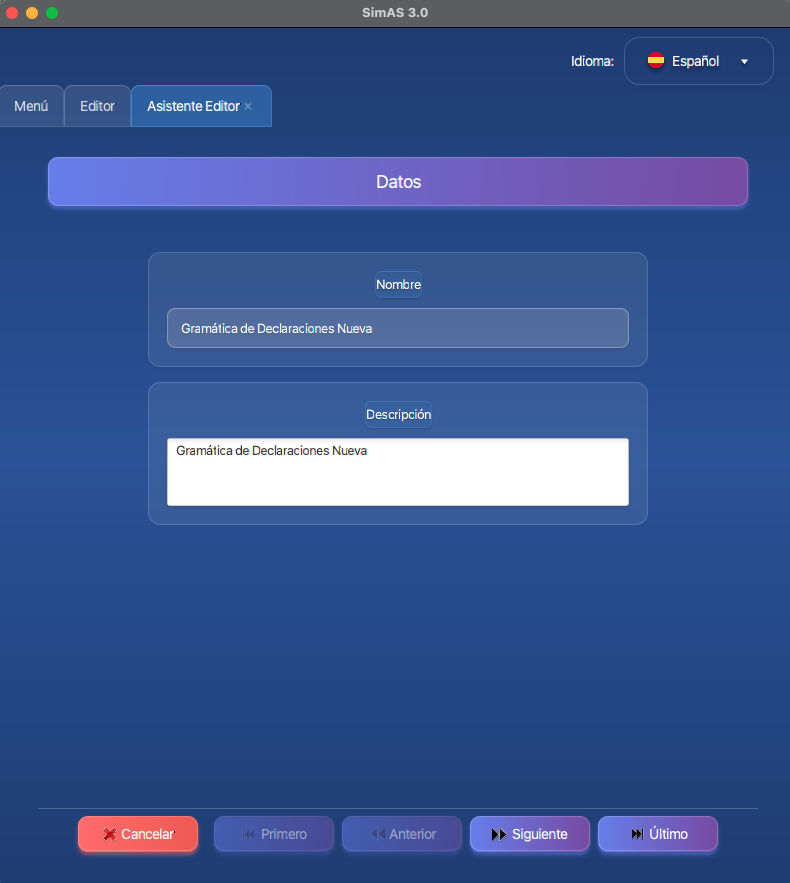
\includegraphics[width=0.9\textwidth]{figuras/ejemplo_practico/editor_paso1.png}
    \caption{Paso 1: Configuración de datos básicos de la gramática}
    \label{fig:ejemplo_editor_paso1}
\end{figure}

En este paso se define:
\begin{itemize}
    \item \textbf{Nombre}: \string"Gramática de Declaraciones Nueva\string"
    \item \textbf{Descripción}: \string"Gramática de Declaraciones Nueva\string"
\end{itemize}

\subsection{Paso 2: Símbolos terminales y no terminales}

El segundo paso implica la definición de todos los símbolos que formarán parte de la gramática. La figura \ref{fig:ejemplo_editor_paso2} muestra la configuración de símbolos:

\needspace{8cm}
\begin{figure}[H]
    \centering
    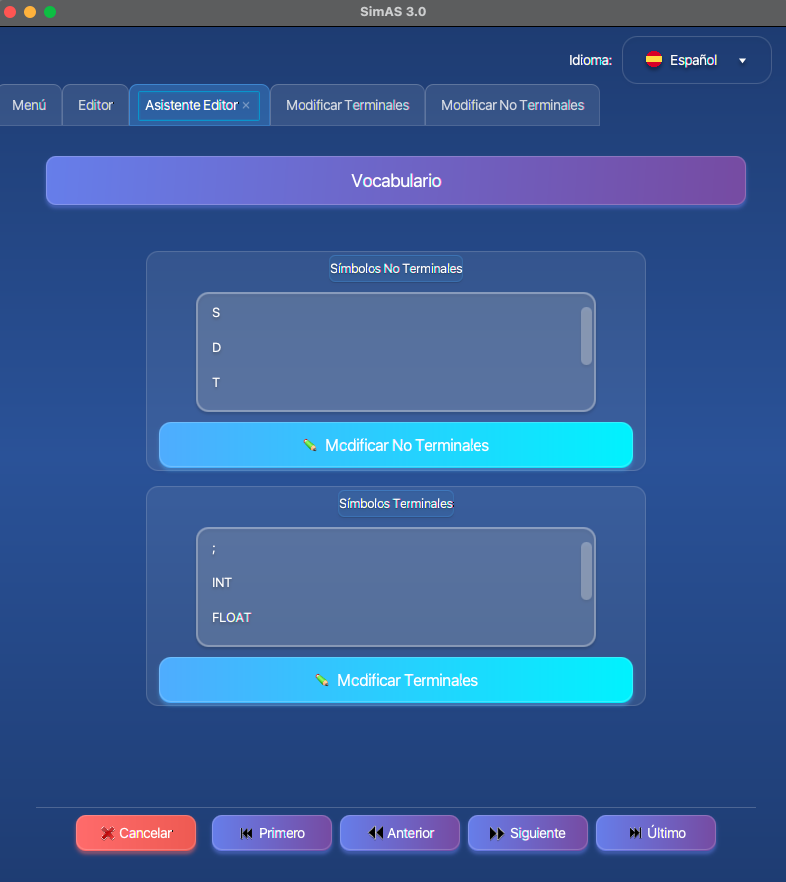
\includegraphics[width=0.9\textwidth]{figuras/ejemplo_practico/editor_paso2.png}
    \caption{Paso 2: Definición de símbolos terminales y no terminales}
    \label{fig:ejemplo_editor_paso2}
\end{figure}

\subsubsection{Símbolos terminales}

Los símbolos terminales definidos incluyen:
\begin{itemize}
    \item \textbf{Tipos de datos}: INT, FLOAT
    \item \textbf{Identificadores}: ID (representando nombres de variables)
    \item \textbf{Separadores}: , (coma), ; (punto y coma)
\end{itemize}

La figura \ref{fig:ejemplo_insertar_terminales} muestra el panel auxiliar para la gestión de símbolos terminales:

\needspace{8cm}
\begin{figure}[H]
    \centering
    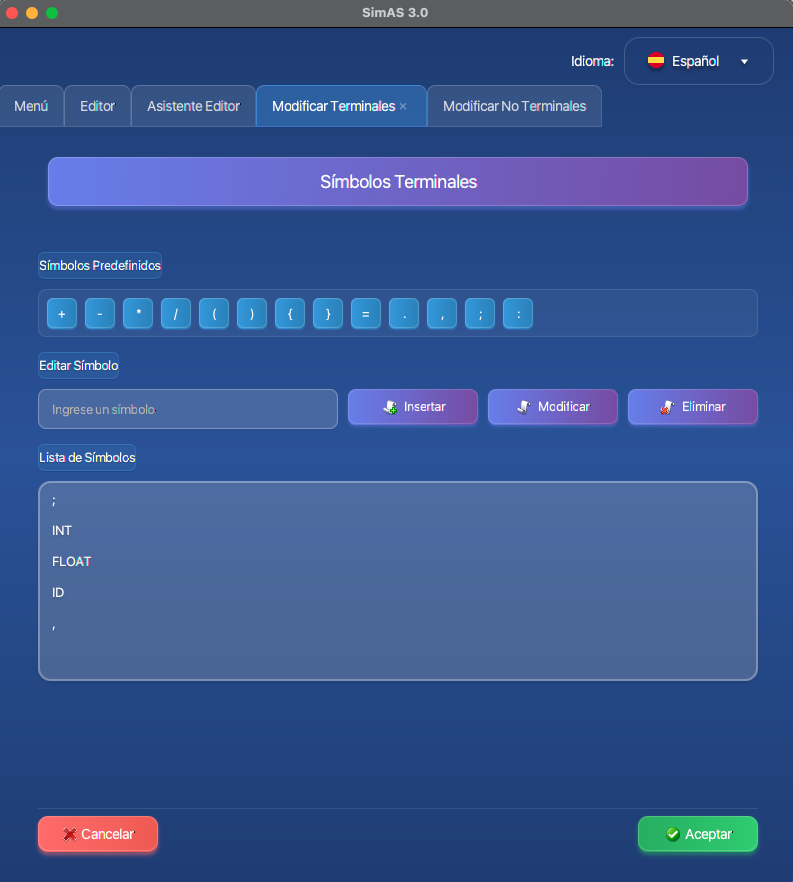
\includegraphics[width=0.9\textwidth]{figuras/ejemplo_practico/insertar_terminales.png}
    \caption{Panel auxiliar para gestión de símbolos terminales}
    \label{fig:ejemplo_insertar_terminales}
\end{figure}

\subsubsection{Símbolos no terminales}

Los símbolos no terminales definidos son:
\begin{itemize}
    \item \textbf{S}: Secuencia de declaraciones
    \item \textbf{D}: Declaración individual
    \item \textbf{T}: Tipo de dato
    \item \textbf{L}: Lista de identificadores
    \item \textbf{L'}: Lista de identificadores (recursiva)
\end{itemize}

La figura \ref{fig:ejemplo_insertar_no_terminales} muestra el panel auxiliar para la gestión de símbolos no terminales:

\needspace{8cm}
\begin{figure}[H]
    \centering
    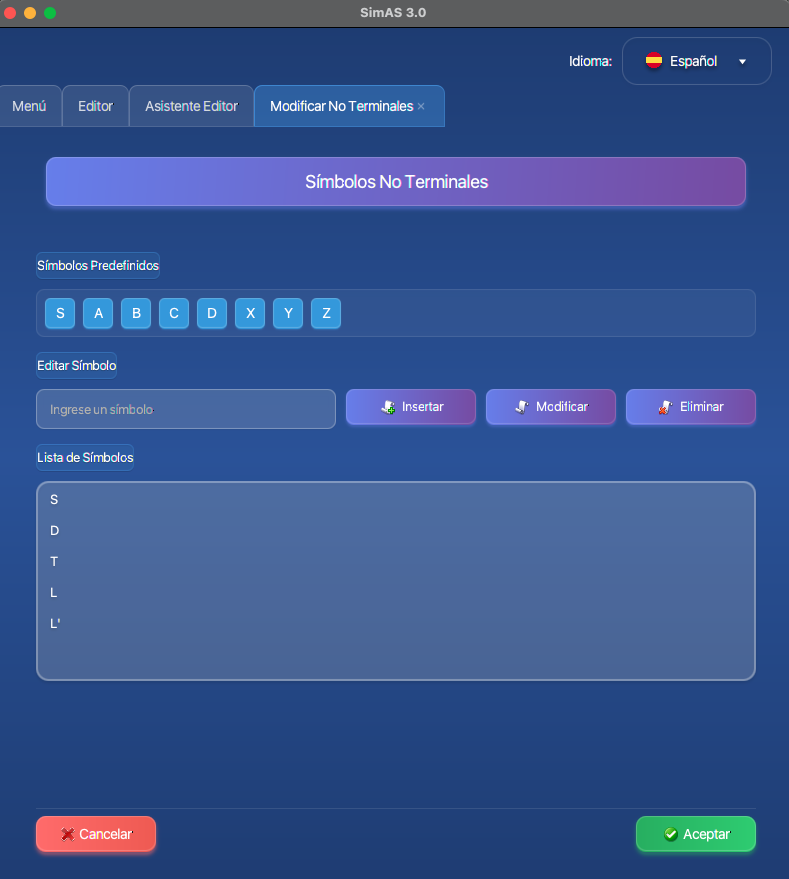
\includegraphics[width=0.9\textwidth]{figuras/ejemplo_practico/insertar_no_terminales.png}
    \caption{Panel auxiliar para gestión de símbolos no terminales}
    \label{fig:ejemplo_insertar_no_terminales}
\end{figure}

\subsection{Paso 3: Producciones}

El tercer paso consiste en definir las reglas de producción de la gramática. La figura \ref{fig:ejemplo_editor_paso3} muestra la configuración de producciones:

\needspace{8cm}
\begin{figure}[H]
    \centering
    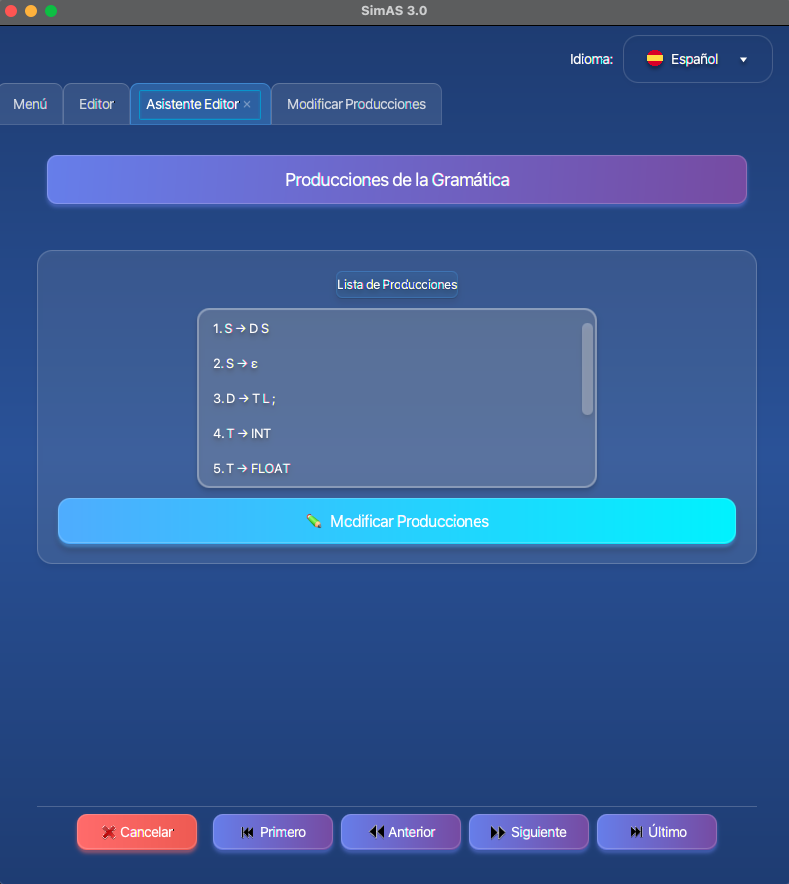
\includegraphics[width=0.9\textwidth]{figuras/ejemplo_practico/editor_paso3.png}
    \caption{Paso 3: Definición de reglas de producción}
    \label{fig:ejemplo_editor_paso3}
\end{figure}

Las producciones definidas para esta gramática son:
\begin{itemize}
    \item S → D S | $\varepsilon$
    \item D → T L ;
    \item T → INT | FLOAT
    \item L → ID L'
    \item L' → , ID L' | $\varepsilon$
\end{itemize}

La figura \ref{fig:ejemplo_insertar_producciones} muestra el panel auxiliar para la gestión de producciones:

\needspace{8cm}
\begin{figure}[H]
    \centering
    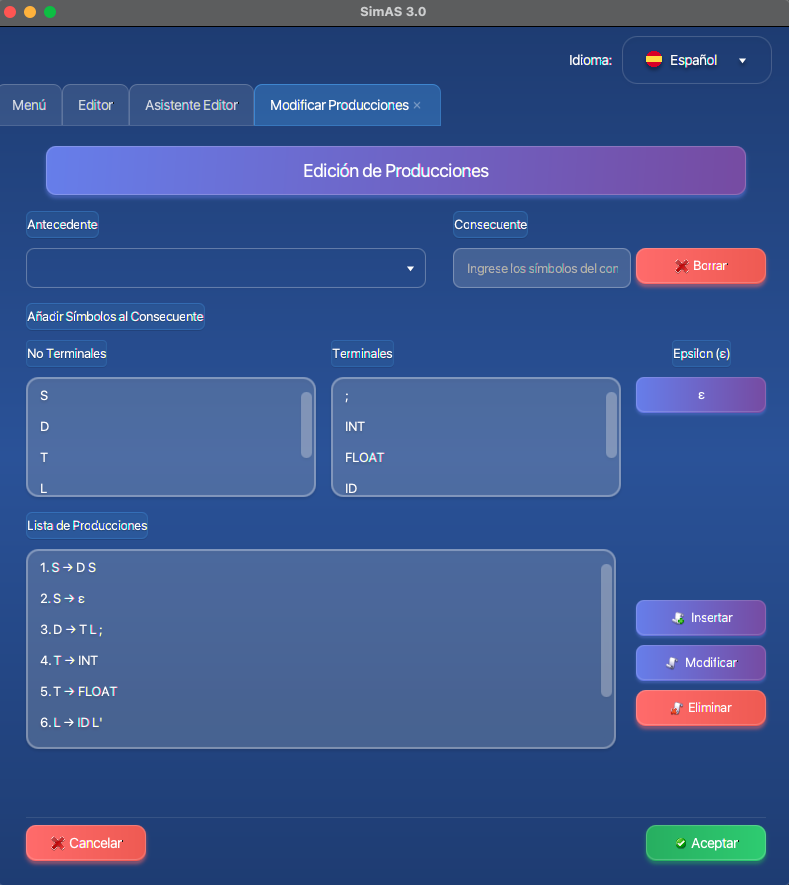
\includegraphics[width=0.9\textwidth]{figuras/ejemplo_practico/insertar_producciones.png}
    \caption{Panel auxiliar para gestión de producciones}
    \label{fig:ejemplo_insertar_producciones}
\end{figure}

\subsection{Paso 4: Símbolo inicial}

El cuarto y último paso del asistente de creación consiste en seleccionar el símbolo inicial de la gramática. La figura \ref{fig:ejemplo_editor_paso4} muestra esta configuración:

\needspace{8cm}
\begin{figure}[H]
    \centering
    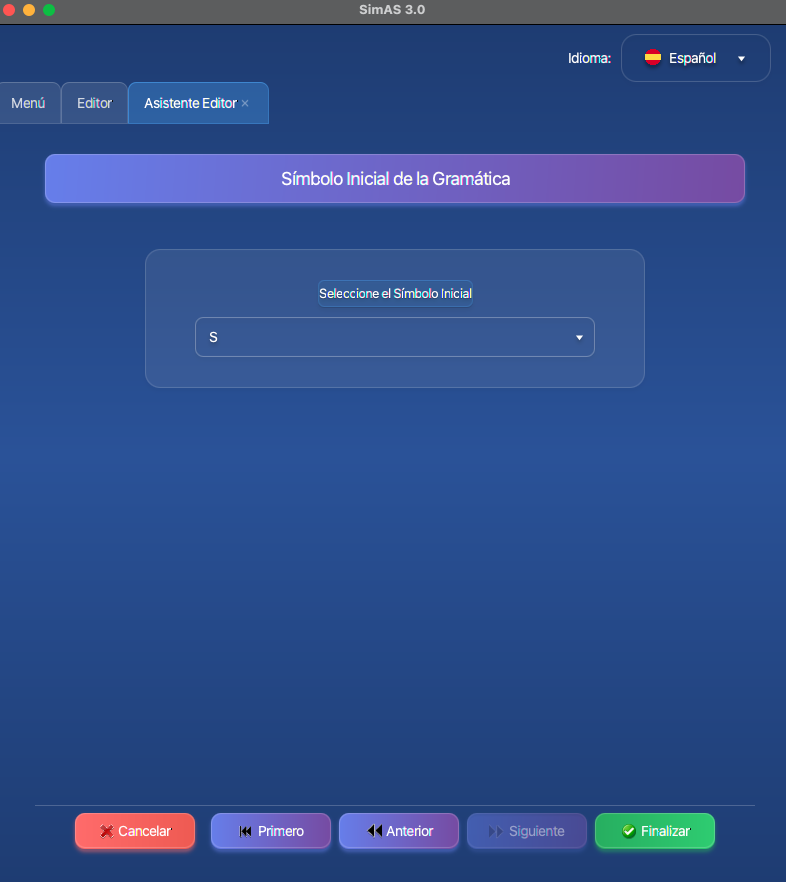
\includegraphics[width=0.9\textwidth]{figuras/ejemplo_practico/editor_paso4.png}
    \caption{Paso 4: Selección del símbolo inicial}
    \label{fig:ejemplo_editor_paso4}
\end{figure}

En este caso, se selecciona \string"S\string" como símbolo inicial, ya que representa la secuencia de declaraciones de la gramática.

\subsection{Validación de la gramática}

Una vez completados todos los pasos, es necesario validar la gramática para asegurar que está correctamente definida. La figura \ref{fig:ejemplo_editor_validar} muestra el resultado de la validación:

\needspace{8cm}
\begin{figure}[H]
    \centering
    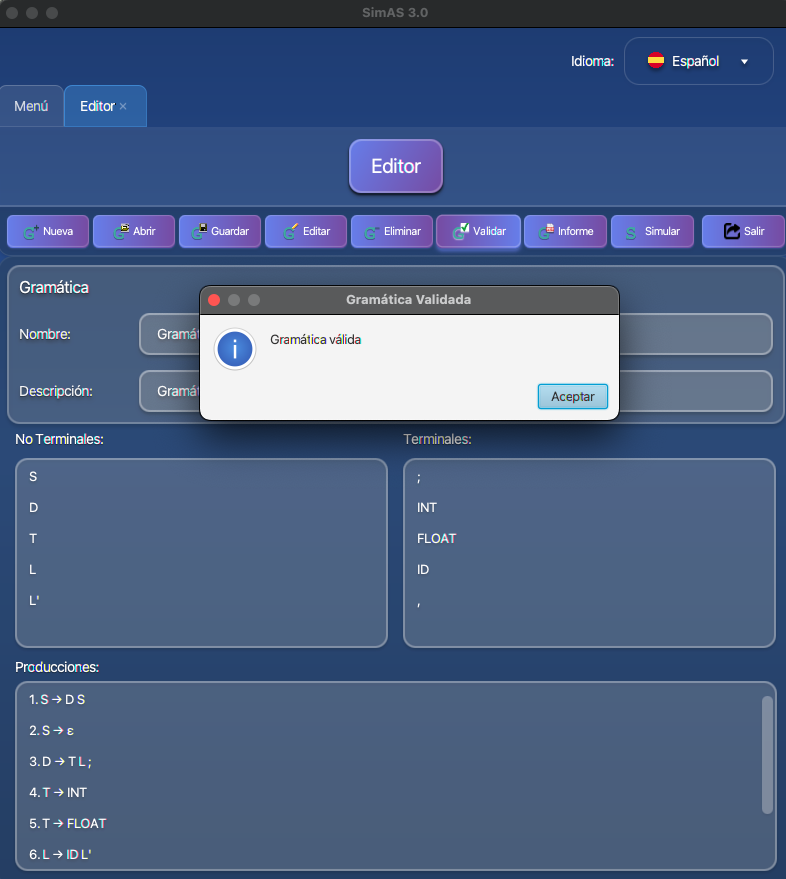
\includegraphics[width=0.9\textwidth]{figuras/ejemplo_practico/editor_validar.png}
    \caption{Validación exitosa de la gramática}
    \label{fig:ejemplo_editor_validar}
\end{figure}

La validación confirma que la gramática está correctamente definida y lista para ser utilizada en el simulador.

\subsection{Vista final del editor}

La figura \ref{fig:ejemplo_editor_final} muestra la vista final del editor con la gramática completamente definida:

\needspace{8cm}
\begin{figure}[H]
    \centering
    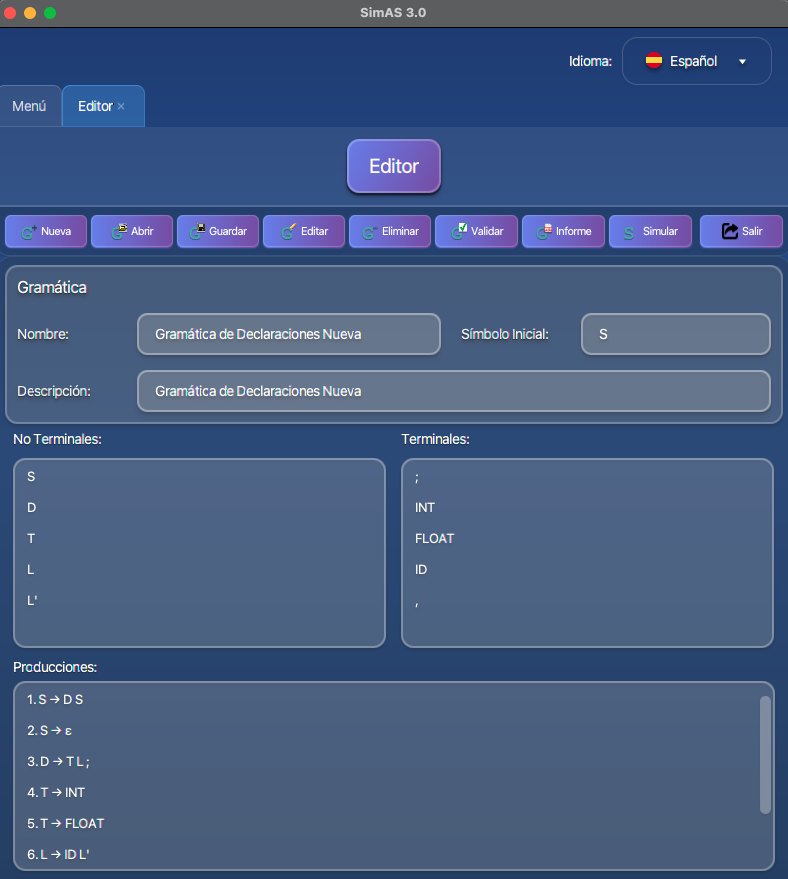
\includegraphics[width=0.9\textwidth]{figuras/ejemplo_practico/editor.png}
    \caption{Vista final del editor con la gramática completa}
    \label{fig:ejemplo_editor_final}
\end{figure}

\section{Simulación del análisis sintáctico descendente}

Una vez creada y validada la gramática, procedemos a utilizar el simulador de análisis sintáctico descendente para analizar cadenas de entrada.

\subsection{Acceso al simulador}

El simulador puede accederse desde el editor utilizando el botón \string"Simular\string", que lleva directamente al paso 1 del asistente de simulación.

\subsection{Paso 1: Refactorización de la gramática}

El primer paso del asistente de simulación consiste en refactorizar la gramática para eliminar la recursividad por la izquierda y factorizar las producciones. La figura \ref{fig:ejemplo_simulador_paso1} muestra este proceso:

\needspace{8cm}
\begin{figure}[H]
    \centering
    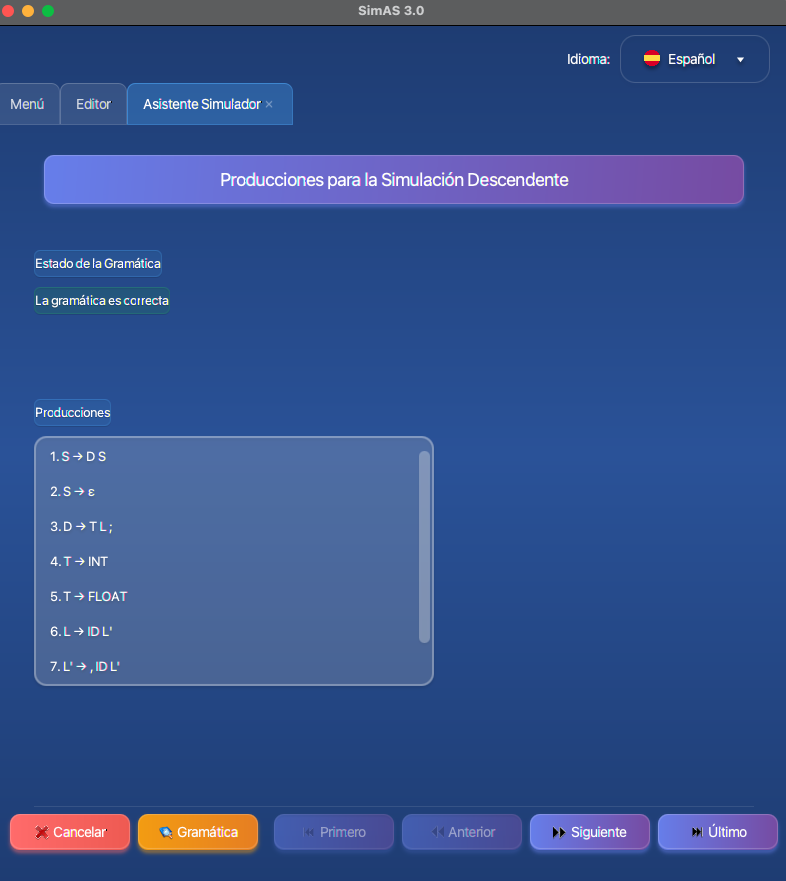
\includegraphics[width=0.9\textwidth]{figuras/ejemplo_practico/simulador_paso1.png}
    \caption{Paso 1: Refactorización de la gramática}
    \label{fig:ejemplo_simulador_paso1}
\end{figure}

La gramática original se transforma para eliminar la recursividad por la izquierda, resultando en:
\begin{itemize}
    \item S → D S | $\varepsilon$
    \item D → T L ;
    \item T → INT | FLOAT
    \item L → ID L'
    \item L' → , ID L' | $\varepsilon$
\end{itemize}

En este caso, la gramática ya está en forma LL(1) y no requiere refactorización adicional, ya que no presenta recursividad por la izquierda.

\subsection{Paso 2: Construcción de conjuntos PRIMERO y SIGUIENTE}

El segundo paso construye automáticamente los conjuntos PRIMERO y SIGUIENTE para cada símbolo no terminal. La figura \ref{fig:ejemplo_simulador_paso2} muestra estos conjuntos:

\needspace{8cm}
\begin{figure}[H]
    \centering
    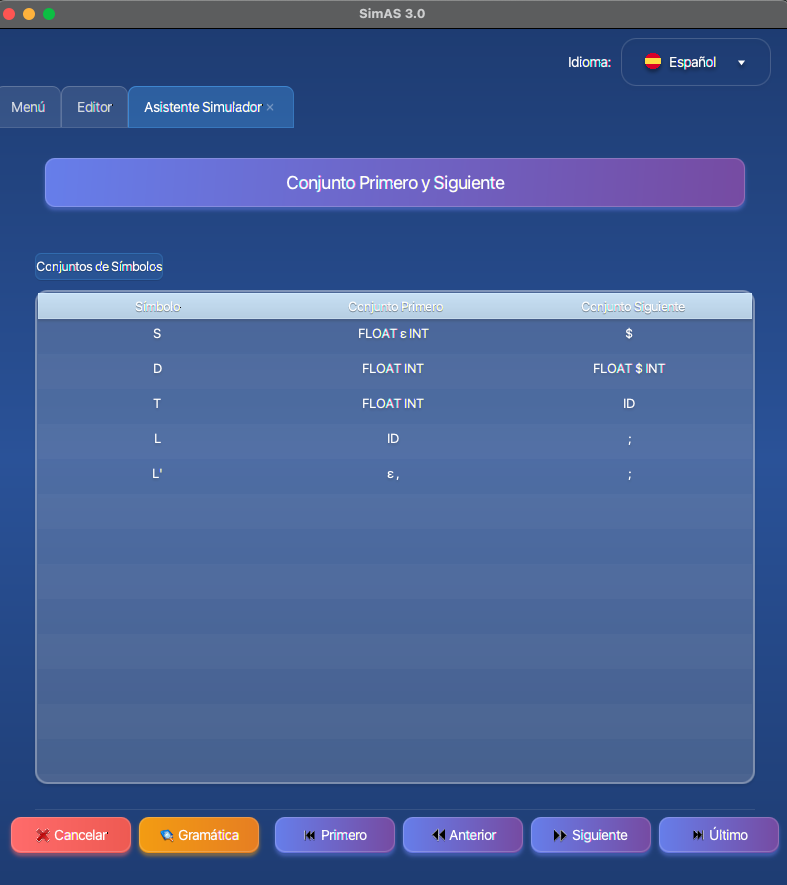
\includegraphics[width=0.9\textwidth]{figuras/ejemplo_practico/simulador_paso2.png}
    \caption{Paso 2: Conjuntos PRIMERO y SIGUIENTE}
    \label{fig:ejemplo_simulador_paso2}
\end{figure}

Los conjuntos calculados son:

\textbf{Conjuntos PRIMERO:}
\begin{itemize}
    \item PRIMERO(S) = \{ INT, FLOAT, $\varepsilon$ \}
    \item PRIMERO(D) = \{ INT, FLOAT \}
    \item PRIMERO(T) = \{ INT, FLOAT \}
    \item PRIMERO(L) = \{ ID \}
    \item PRIMERO(L') = \{ ,, $\varepsilon$ \}
\end{itemize}

\textbf{Conjuntos SIGUIENTE:}
\begin{itemize}
    \item SIGUIENTE(S) = \{ \$ \}
    \item SIGUIENTE(D) = \{ INT, FLOAT, \$ \}
    \item SIGUIENTE(T) = \{ ID \}
    \item SIGUIENTE(L) = \{ ; \}
    \item SIGUIENTE(L') = \{ ; \}
\end{itemize}

\subsection{Paso 3: Construcción de la tabla predictiva}

El tercer paso genera la tabla predictiva basada en los conjuntos PRIMERO y SIGUIENTE. La figura \ref{fig:ejemplo_simulador_paso3} muestra la tabla resultante:

\needspace{8cm}
\begin{figure}[H]
    \centering
    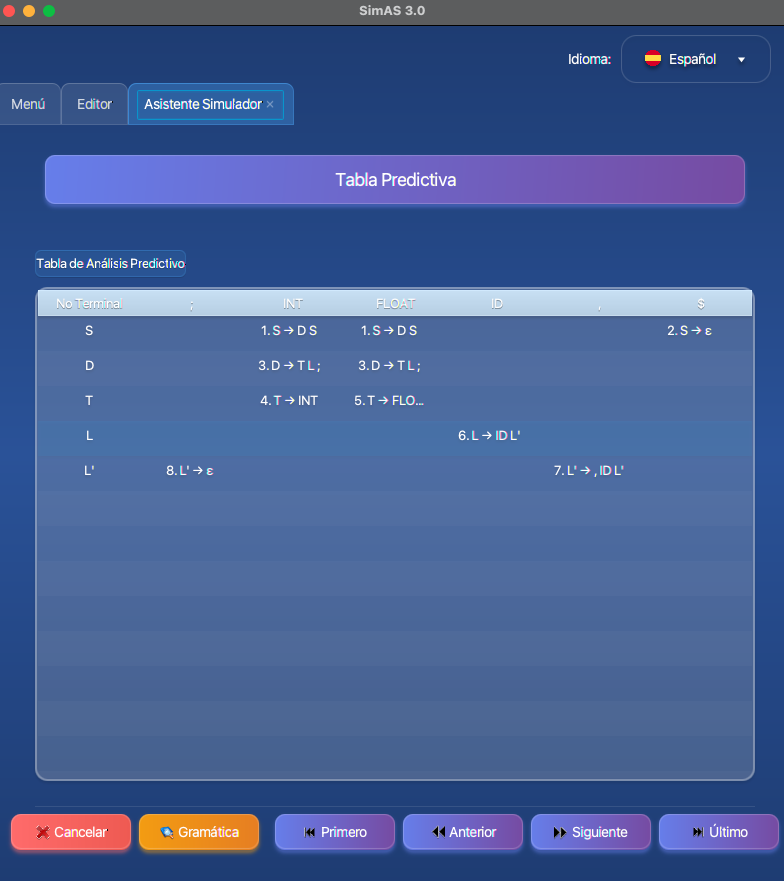
\includegraphics[width=0.9\textwidth]{figuras/ejemplo_practico/simulador_paso3.png}
    \caption{Paso 3: Tabla predictiva}
    \label{fig:ejemplo_simulador_paso3}
\end{figure}

\subsection{Paso 4: Funciones de error}

El cuarto paso permite configurar funciones de error para el manejo de cadenas incorrectas. La figura \ref{fig:ejemplo_simulador_paso4} muestra la configuración de funciones de error:

\needspace{8cm}
\begin{figure}[H]
    \centering
    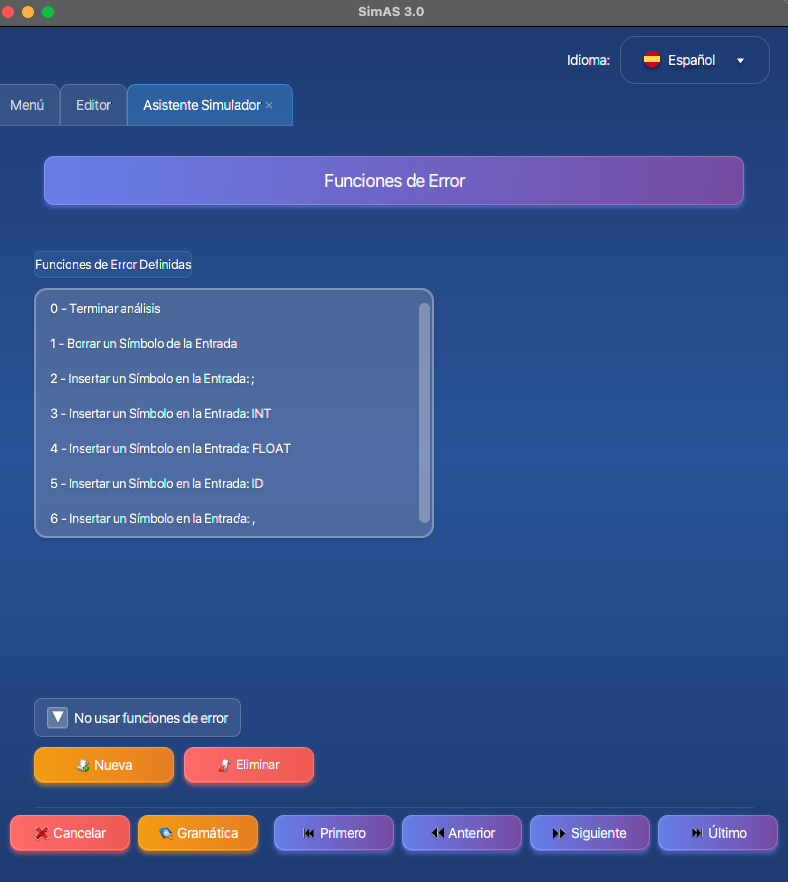
\includegraphics[width=0.9\textwidth]{figuras/ejemplo_practico/simulador_paso4.png}
    \caption{Paso 4: Configuración de funciones de error}
    \label{fig:ejemplo_simulador_paso4}
\end{figure}

La figura \ref{fig:ejemplo_insertar_funcion_error} muestra el panel auxiliar para añadir nuevas funciones de error:

\needspace{8cm}
\begin{figure}[H]
    \centering
    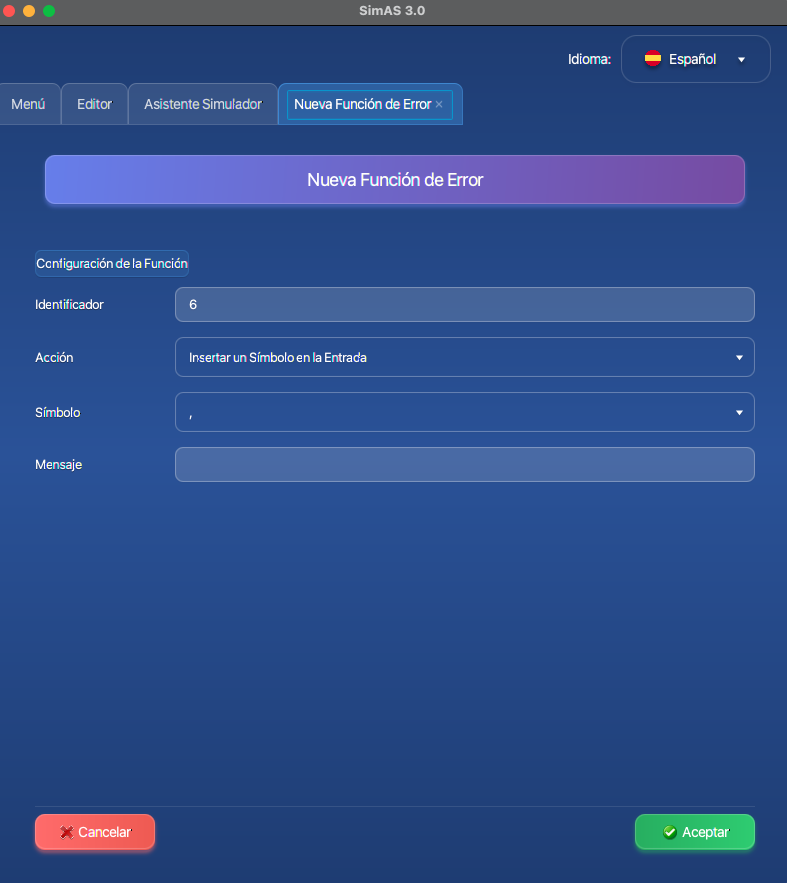
\includegraphics[width=0.9\textwidth]{figuras/ejemplo_practico/insertar_funcion_error.png}
    \caption{Panel auxiliar para añadir funciones de error}
    \label{fig:ejemplo_insertar_funcion_error}
\end{figure}

\subsection{Paso 5: Tabla predictiva completa}

El quinto paso presenta la tabla predictiva completa con todas las funciones de error configuradas. La figura \ref{fig:ejemplo_simulador_paso5} muestra esta tabla final:

\needspace{8cm}
\begin{figure}[H]
    \centering
    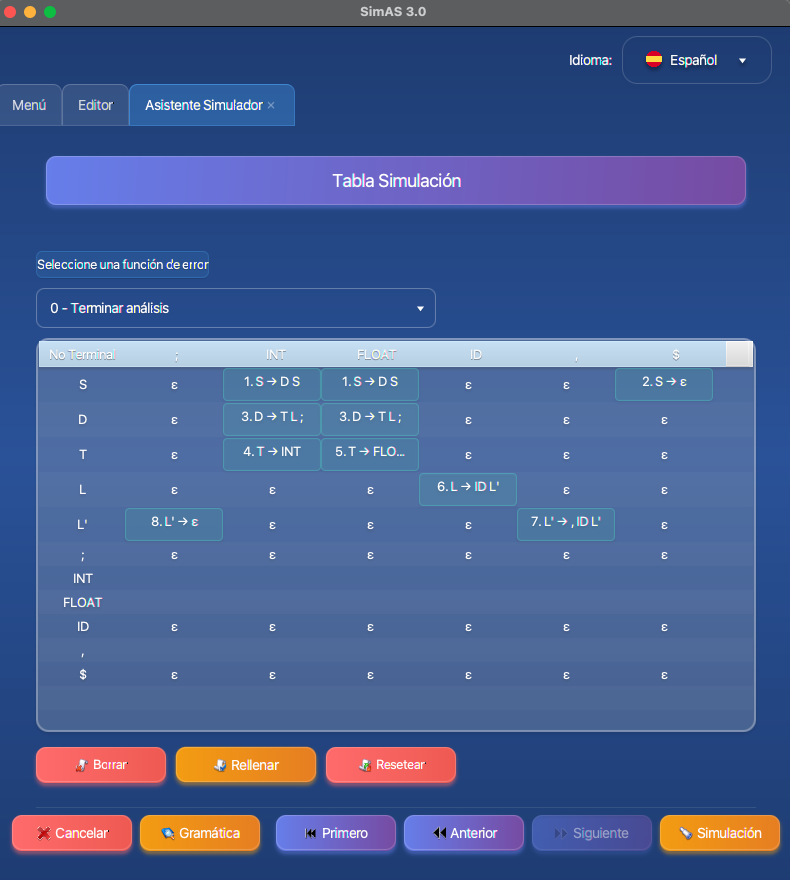
\includegraphics[width=0.9\textwidth]{figuras/ejemplo_practico/simulador_paso5.png}
    \caption{Paso 5: Tabla predictiva completa}
    \label{fig:ejemplo_simulador_paso5}
\end{figure}

Una vez completada la configuración de la tabla predictiva, se puede proceder al simulador principal haciendo clic en el botón \string"Simulación\string". Desde el simulador principal se accede a la simulación interactiva.

\subsection{Simulador principal}

El simulador principal muestra un resumen completo de la configuración realizada, incluyendo las producciones modificadas, las funciones de error configuradas y la tabla predictiva completa. La figura \ref{fig:ejemplo_simulador_principal} muestra la interfaz del simulador principal:

\needspace{8cm}
\begin{figure}[H]
    \centering
    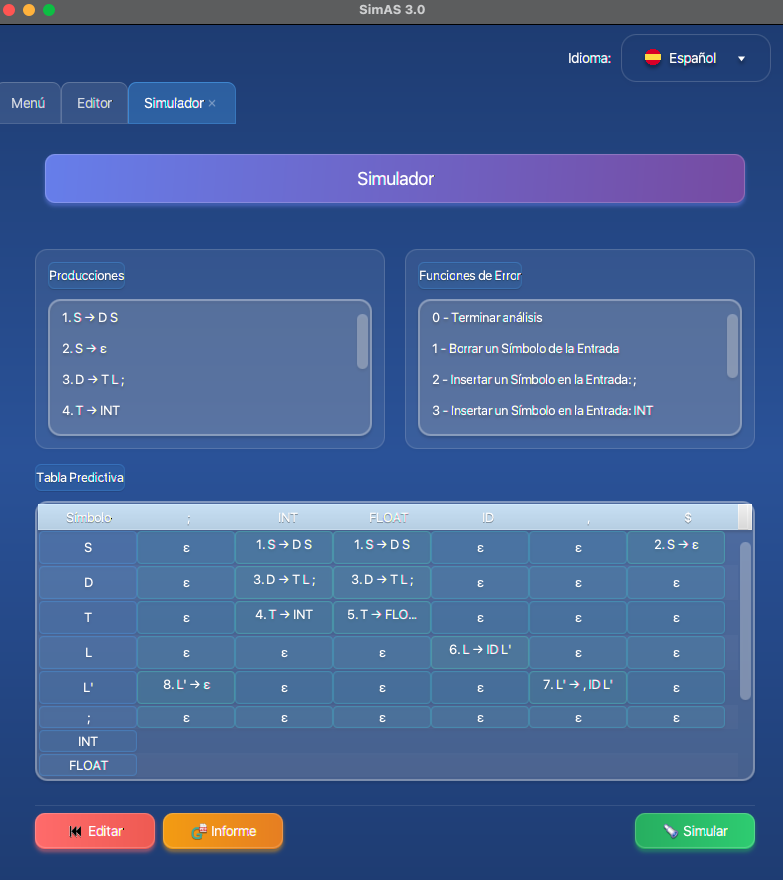
\includegraphics[width=0.9\textwidth]{figuras/ejemplo_practico/simulador.png}
    \caption{Simulador principal con resumen de configuración}
    \label{fig:ejemplo_simulador_principal}
\end{figure}

Desde este simulador se puede generar un informe PDF con toda la información y acceder a la simulación interactiva.

\subsection{Simulación interactiva}

Desde el simulador principal, haciendo clic en el botón \string"Simular\string", se accede a la simulación interactiva. La figura \ref{fig:ejemplo_simulacion_cadena} muestra la introducción de una cadena de entrada:

\needspace{8cm}
\begin{figure}[H]
    \centering
    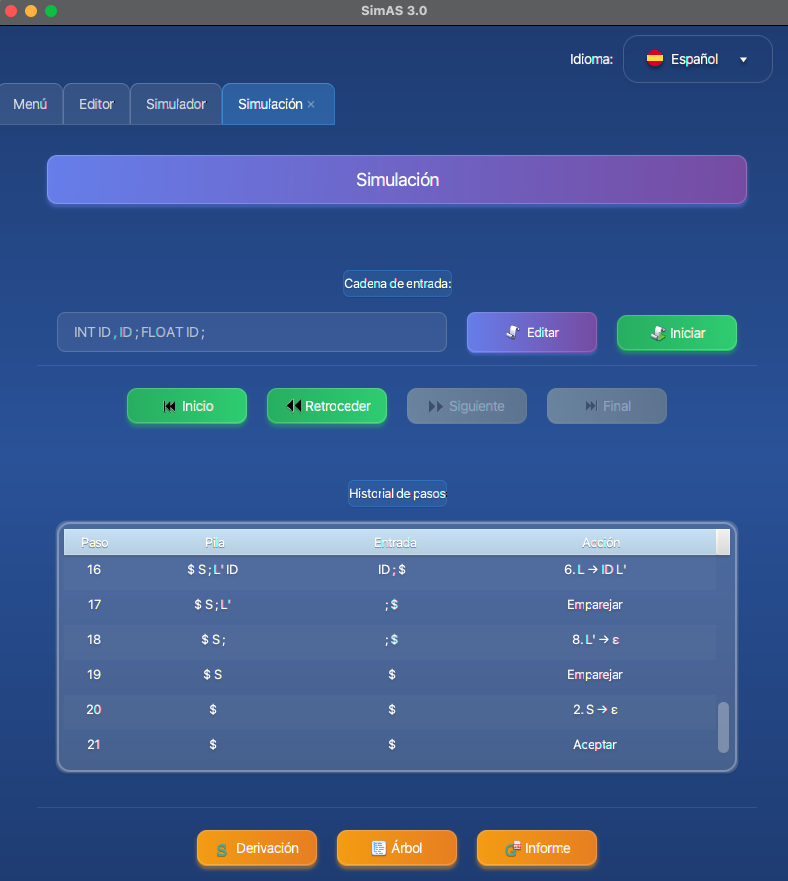
\includegraphics[width=0.9\textwidth]{figuras/ejemplo_practico/simulacion_cadena1.png}
    \caption{Introducción de cadena de entrada para simulación}
    \label{fig:ejemplo_simulacion_cadena}
\end{figure}

Para este ejemplo, utilizaremos la cadena \string"INT x, y;\string" que representa la declaración de dos variables enteras.

\subsection{Derivación de la simulación}

La figura \ref{fig:ejemplo_simulacion_derivacion} muestra la derivación paso a paso del análisis sintáctico:

\needspace{8cm}
\begin{figure}[H]
    \centering
    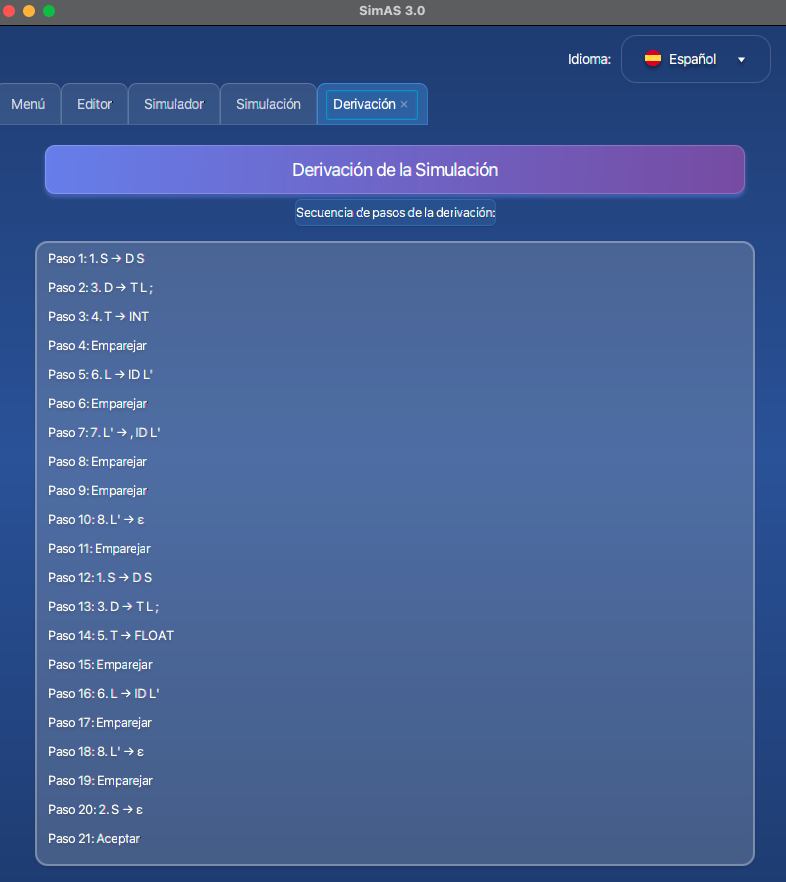
\includegraphics[width=0.9\textwidth]{figuras/ejemplo_practico/simulacion_derivacion1.png}
    \caption{Derivación paso a paso del análisis sintáctico}
    \label{fig:ejemplo_simulacion_derivacion}
\end{figure}

La derivación muestra cómo se aplican las reglas de producción para reconocer la cadena de entrada, comenzando con el símbolo inicial S y aplicando las reglas correspondientes según la tabla predictiva.

\subsection{Árbol de análisis sintáctico}

La figura \ref{fig:ejemplo_simulacion_arbol} muestra el árbol de análisis sintáctico generado:

\needspace{8cm}
\begin{figure}[H]
    \centering
    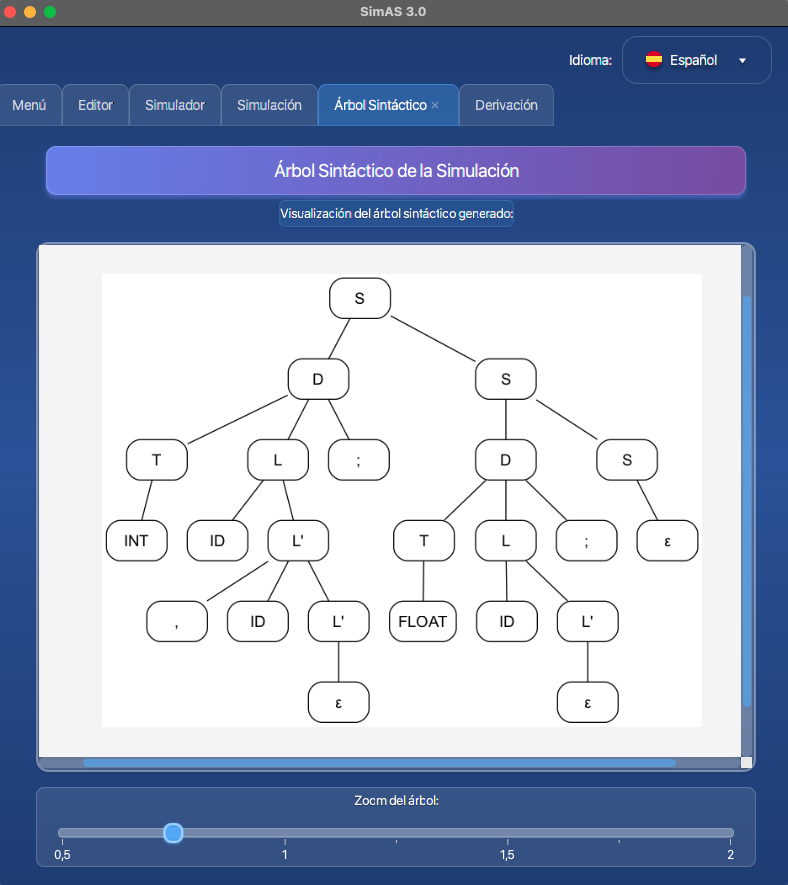
\includegraphics[width=0.9\textwidth]{figuras/ejemplo_practico/simulacion_arbol1.png}
    \caption{Árbol de análisis sintáctico}
    \label{fig:ejemplo_simulacion_arbol}
\end{figure}

El árbol muestra la estructura jerárquica de la declaración, donde se puede observar cómo se organizan los elementos: el tipo de dato (INT), seguido de la lista de identificadores (x, y) y el punto y coma final.

\section{Conclusión del ejemplo}

Este ejemplo práctico ha demostrado el flujo completo de trabajo con SimAS 3.0:

\begin{enumerate}
    \item \textbf{Creación de gramática}: Se utilizó el editor guiado para crear una gramática de declaraciones de variables.
    \item \textbf{Validación}: Se verificó que la gramática estuviera correctamente definida.
    \item \textbf{Refactorización}: Se confirmó que la gramática ya estaba en forma LL(1) sin recursividad por la izquierda.
    \item \textbf{Construcción de tablas}: Se generaron automáticamente los conjuntos PRIMERO y SIGUIENTE, y la tabla predictiva.
    \item \textbf{Configuración de errores}: Se establecieron funciones de error para el manejo de cadenas incorrectas.
    \item \textbf{Simulación}: Se realizó un análisis sintáctico completo de una declaración de variables.
    \item \textbf{Visualización}: Se generaron la derivación y el árbol de análisis sintáctico.
\end{enumerate}

Este proceso ilustra cómo SimAS 3.0 facilita el aprendizaje y comprensión de los conceptos fundamentales del análisis sintáctico descendente, proporcionando herramientas visuales e interactivas que hacen accesible este tema complejo de la teoría de lenguajes formales.
